\tikzstyle{line} = [draw, -latex]
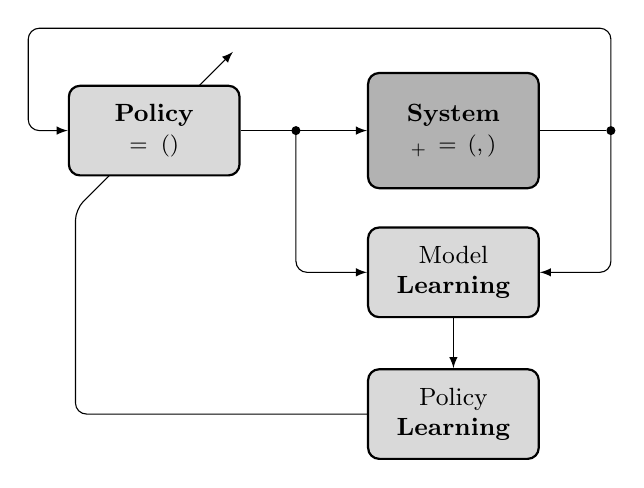
\begin{tikzpicture}[rounded corners, text centered]
\tikzstyle{dot} = [circle, draw, fill=black, inner sep=1pt]
  \small
  \node[draw, fill=black!15, thick, text width=6em, minimum height=3.5em] at (0,-3.6) (pilco){Policy \bf Learning};
  \path[line] (pilco.west) -| (-4.8,-1.0) -- (-2.8,1.0);

  \node[draw, thick, fill=black!15, text width=6em, minimum height=3.5em] at (-3.8,0) (pol){\bf Policy  \\ {\footnotesize $\bu = \bpi(\bx)$}};
  \node[draw, thick, fill=black!30, text width=6em, minimum height=4.5em] at (0,0) (sys){\bf System \\ {\footnotesize $\bx_+ = \bff(\bx,\bu)$}};
  \node[draw, thick, fill=black!15, text width=6em, minimum height=3.5em] at (0,-1.8) (GP){Model \bf Learning};
  
  \node[dot] at (-2,0) (dot1){};
  \node[dot] at (2,0) (dot2){};

  \path[draw] (sys.east) -- (dot2);
  \path[line] (dot2) |- (-5.4,1.3) |- (pol.west);
  \path[line] (pol.east) -- (sys.west);
  \path[line] (dot1) |- (GP.west);
  \path[line] (dot2) |- (GP.east);
  \path[line] (GP.south) -- (pilco.north);

  \node at (1.6,0.2) {$\bx$};
  \node at (-2,0.2) {$\bu$};
  %\node at (0.6,-2.85) {$\EE[\bw]$};
  \node at (-4.4,-3.35) {$\bpsi$};

\end{tikzpicture}
